%!TEX root = ../thesis.tex
\chapter{The one with cross entropy \label{ch:crossentropy}}


We can calculate...




Recall \autoref{eq:entropyrate}, which while a useful theoretical tool, can be very difficult to compute.


\begin{definition}
	For a stochastic process $\mathcal{X} = \{X_i\}$, with a realisation of $n$ states and a finite alphabet,  the entropy rate can be estimated using,
		\begin{equation}\label{eq:estimate}
	H(\mathcal{X}) \approx\frac{|\mathcal{X}| \log |\mathcal{X}| }{\sum_{i=0}^n \Lambda_{i} }
	\end{equation}
	Where $|\mathcal{X}|$ is the size of the alphabet and $\Lambda_{i}$ is the length of the shortest subsequence starting at position $i$ that does not appear as a contiguous subsequence in the previous $i$ symbols $X_{0}^{i}$. This can also be obtained by adding 1 to the longest match-length, 
	 \begin{equation}
	  \Lambda_{i}=1+\max \left\{l: X_{i}^{i+l}=X_{j}^{j+l}, 0 \leq j \leq N-i, 0 \leq l \leq N - i - j \right\}
	 \end{equation}
\end{definition}






% test what suffiently long means in complexity ( plot of complexity vs speed of convegence)


\resizebox{1\textwidth}{!}{
	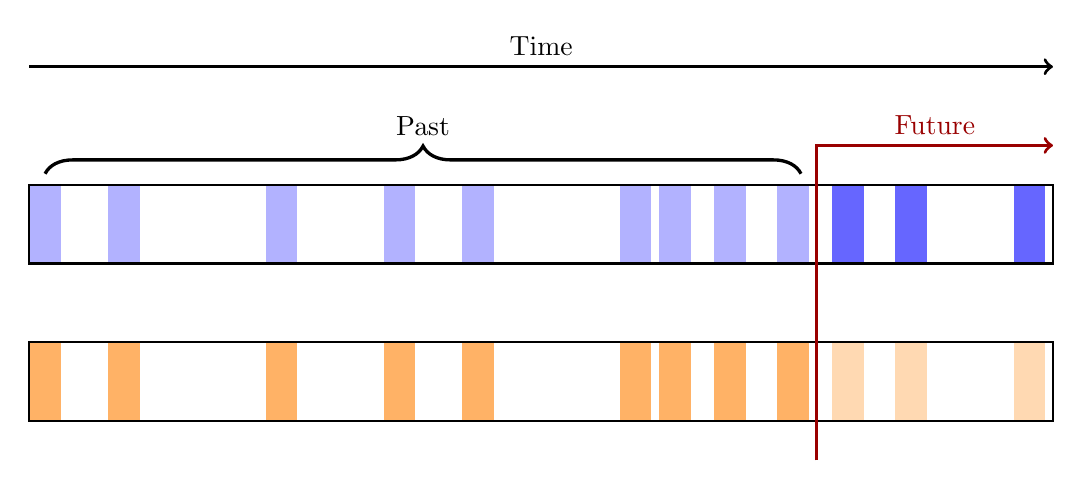
\begin{tikzpicture}
	
	%% BLUE EVENTS
	% Main
	\draw [thick] (0,0) rectangle (13,1) ;
	
	% Events
	% Past Events
	\foreach \x in {0, 1, 3, 4.5, 5.5, 7.5, 8, 8.7, 9.5}
	{
		\fill[blue!30!white] (\x,0) rectangle ++(0.4,1);
	}
	% Future Events
	\foreach \x in {10.2, 11, 12.5}
	{
		\fill[blue!60!white] (\x,0) rectangle ++(0.4,1);
	}
	
	% Redraw Main Rectangle
	\draw [thick] (0,0) rectangle (13,1) ;
	
	
	%%ORANGE EVENTS
	
	% Main
	\draw [thick] (0,0) rectangle (13,1) ;
	
	% Events
	% Past Events
	\foreach \x in {0, 1, 3, 4.5, 5.5, 7.5, 8, 8.7, 9.5}
	{
		\fill[orange!60!white] (\x,-2) rectangle ++(0.4,1);
	}
	% Future Events
	\foreach \x in {10.2, 11, 12.5}
	{
		\fill[orange!30!white] (\x,-2) rectangle ++(0.4,1);
	}
	
	% Redraw Main Rectangle
	\draw [thick] (0,-2) rectangle (13,-1) ;
	
	
	
	
	% Future
	\draw [red!60!black, very thick, shorten >= -0.6pt]        (10,-2.5 ) -- (10,1.5);
	\draw [red!60!black, very thick, ->] (10,   1.5)  -- (13, 1.5)   node[midway, above] {Future} ;
	
	% Time Arrow
	\draw [very thick, ->] (0,2.5) -- (13,2.5) node[midway, above] {Time} ;
	
	% Past brace
	\usetikzlibrary{decorations.pathreplacing}
	\draw [very thick, -, draw=black, decorate, decoration={brace,amplitude=10pt,mirror,raise=4pt} ] (9.8,1) -- (0.2,1)
	node[midway, above, yshift = 14pt] {Past} ;
	
	\end{tikzpicture}
}



old

\resizebox{1\textwidth}{!}{
	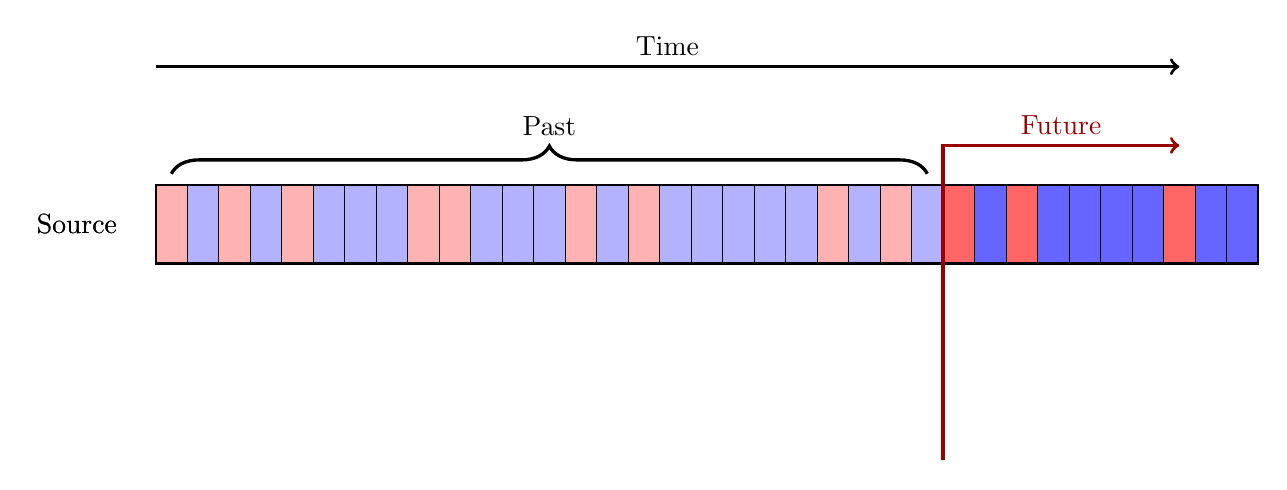
\begin{tikzpicture}
	
	%% TOP EVENTS
	
	\node at (-1, 0.5) {Source};
	
	% Events
	% Past Events
	\draw [thick, fill = blue!30!white] (0,0)  rectangle (10,1)  ;
	\foreach \x in {0, 0.8, 1.6, 3.2, 3.6, 5.2, 6, 8.4, 9.2}
	{
		\fill[red!30!white] (\x ,0) rectangle ++(0.4,1);
	}
	
	% Future Events
	\draw [thick, fill = blue!60!white] (10,0) rectangle (14,1) ;
	\foreach \x in {10, 10.8, 12.8}
	{
		\fill[red!60!white] (\x,0) rectangle ++(0.4,1);
	}
	
	% Redraw Main Rectangle
	\foreach \x in {0,...,34}
	{
		\draw [very thin] (0.4*\x,0)  rectangle ++(0.4,1);
	}
	\draw [thick] (0,0) rectangle (14,1) ;
	
	
	
	%%ORANGE EVENTS
	
	\node at (-1, 0.5) {Source};
	
	% Events
	% Past Events
	\draw [thick, fill = blue!30!white] (0,0)  rectangle (10,1)  ;
	\foreach \x in {0, 0.8, 1.6, 3.2, 3.6, 5.2, 6, 8.4, 9.2}
	{
		\fill[red!30!white] (\x ,0) rectangle ++(0.4,1);
	}
	
	% Future Events
	\draw [thick, fill = blue!60!white] (10,0) rectangle (14,1) ;
	\foreach \x in {10, 10.8, 12.8}
	{
		\fill[red!60!white] (\x,0) rectangle ++(0.4,1);
	}
	
	% Redraw Main Rectangle
	\foreach \x in {0,...,34}
	{
		\draw [very thin] (0.4*\x,0)  rectangle ++(0.4,1);
	}
	\draw [thick] (0,0) rectangle (14,1) ;
	
	
	
	% Future
	\draw [red!60!black, very thick, shorten >= -0.6pt]        (10,-2.5 ) -- (10,1.5);
	\draw [red!60!black, very thick, ->] (10,   1.5)  -- (13, 1.5)   node[midway, above] {Future} ;
	
	% Time Arrow
	\draw [very thick, ->] (0,2.5) -- (13,2.5) node[midway, above] {Time} ;
	
	% Past brace
	\usetikzlibrary{decorations.pathreplacing}
	\draw [very thick, -, draw=black, decorate, decoration={brace,amplitude=10pt,mirror,raise=4pt} ] (9.8,1) -- (0.2,1)
	node[midway, above, yshift = 14pt] {Past} ;
	
	\end{tikzpicture}
}